\documentclass[__main__.tex]{subfiles}

\begin{document}

\title{О}{10}
Классификация дифракционных явлений. Дифракция Фраунгофера на длинной прямоугольной щели. Влияние ширины щели на дифракционную картину.\\ 


\textbf{Классификация дифракционных явлений}\\

Если диафрагма закрыта, то понятно, что за ней нет никакой волны. Будем постепенно ее открывать. В точке наблюдения будет монотонно расти освещенность. В этой области ($m << 1$) на оси ничего интересного не происходит, но на экране наблюдаются кольца – дифракция уже есть и в этих условиях, она называется дифракцией Фраунгофера.
Мы уже устремили источник в бесконечность. Если $m << 1$,
то и точка наблюдения очень далеко ($b \rightarrow \infty$). На диафрагму падает почти параллельный пучок света, и за диафрагмой распространяются лучи параллельные лучи в различных направлениях. Поэтому дифракцию Фраунгофера еще называют дифракцией в параллельных лучах.\\
Так будет продолжаться до тех пор, пока число $m$ не станет равным единице – это максимум, соответствующий одной открытой зоне Френеля. Далее последует минимум с почти нулевой интенсивностью (две открытые зоны), и затем максимумы, уменьшаясь по интенсивности, будут чередоваться с минимумами, которые все больше и больше будут отличаться от нуля. Дифракция в условиях, когда число $m$ равняется нескольким единицам, называется дифракцией Френеля.
Наконец, при дальнейшем увеличении радиуса диафрагмы интенсивность становится равной интенсивности в отсутствие преград, лучи распространяются прямолинейно, так что при $m >> 1$ мы переходим в область геометрической
оптики.\\

\textbf{Дифракция Фраунгофера на длинной прямоугольной щели: схема наблюдения, влияние ширины щели на дифракционную картину, условия наблюдения дифракции.}\\

\begin{figure}[h]
	\begin{center}
		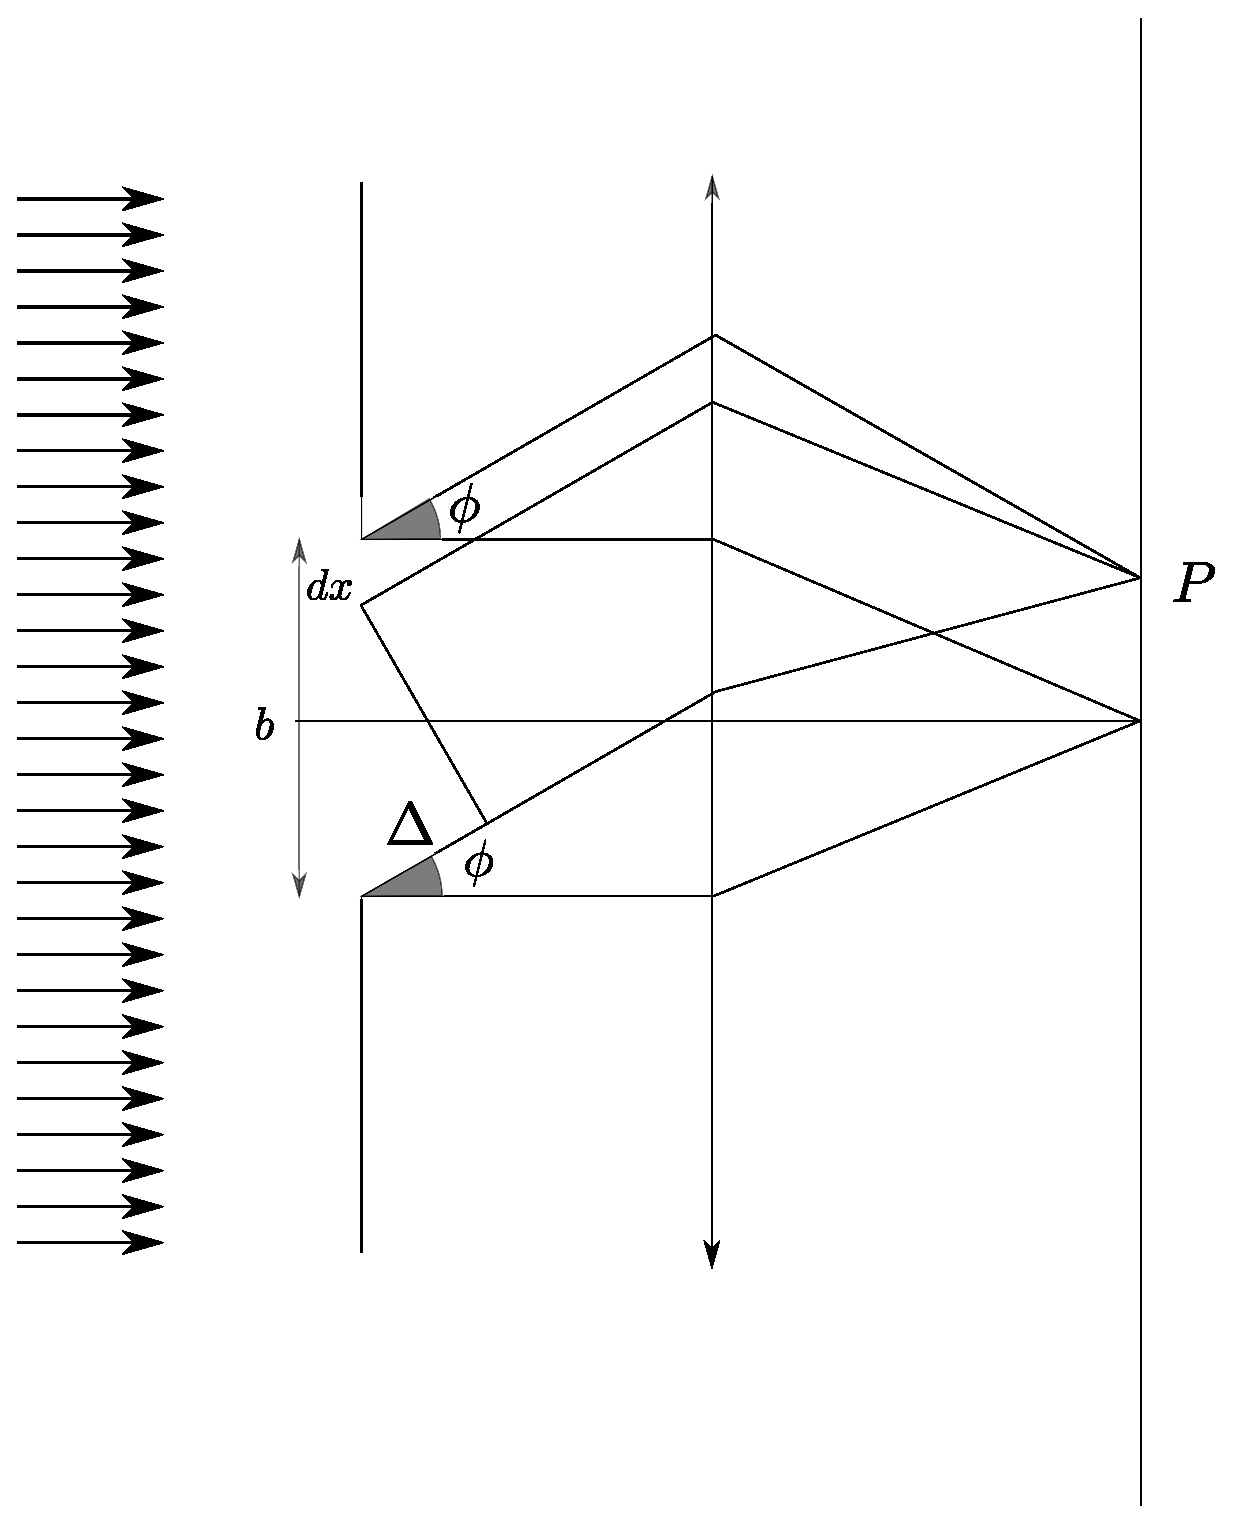
\includegraphics[width=0.5\linewidth]{img/o-08_3.eps}
	\end{center}
\end{figure}

Дифракция Фраунгофера, как уже говорилось, это дифракция в параллельных лучах. Параллельный пучок света падает нормально на плоский экран со щелью шириной $b$ – и то, и другое перпендикулярно плоскости рисунка. За щелью расположена линза Л, в фокальной плоскости которой находится экран Э. Параллельные лучи, идущие от разных полос щели, собираются в полосы на экране. Например, элемент рисунка $dx$ представляет бесконечно узкую полосу. Идущие от нее лучи, перпендикулярные плоскости щели, собираются в центральную полосу, а лучи, идущие под углом $\phi$ к нормали – в точку $P$, которая также представляет целую полосу (точнее, линию) экрана Э, перпендикулярную плоскости рисунка. Далее мы будем просто говорить «точка», имея в виду, что во всех плоскостях, параллельных плоскости рисунка, все происходит в точности так же.
От всех элементов щели $dx$ лучи расходятся по всем направлениям, но в отличие от дифракции Френеля их можно считать плоскими волнами. Фазы и амплитуды колебаний во всех точках щели одинаковы.
Линза обладает важным свойством – она не вносит дополнительной разности фаз в падающие на нее параллельные лучи, которые собираются в фокальной
плоскости. Однако у лучей, идущих от различных элементов щели есть оптическая разность хода. Оптическая разность хода между лучом, идущим из элемента $dx$, и лучом от нижней точки щели О под углом $\phi$ к нормали равна $\Delta = x\sin\phi$\\
Если ширина щели меньше длины волны, то ничего не видно, кроме нулевого максимума – дифракционной картины как таковой нет.
Чем шире щель, тем\\
1) ярче картина\\
2) меньше контрастность\\
3) уже линии\\
4) больше число максимумов\\.
\\
Перечислим условия, при которых можно наблюдать дифракцию.
Поперечный размер объекта $b$ должен быть больше длины волны, $b > \lambda$ , но не может быть и слишком большим, так как\\
1) необходимо выполнения условия пространственной (поперечной) когерентности $b<\rho_{\text{когер}}$ ,\\
2) должно выполняться условие временной (продольной) когерентности $b\sin\phi < \frac{\lambda^2}{\delta \lambda}$. В роли ширины спектра $\delta\lambda$ может выступать цветовое разрешение глаза\\
3) если значение $m_{max}$ велико, то картина теряет контрастность; при этом может еще быть наблюдаемой дифракция Френеля, либо вообще речь уже
идет о геометрической оптике.
\end{document} 


